

\begin{multicols}{2}
\subsection*{Presented}
\begin{itemize}
    \item BEER algorithm \ref{alg:ben-tile}  by Xiaobai
    \item BEN (not done yet)
    \item 
    \item \juntang[inline]{TBP: BEN improved}
\end{itemize}

\subsection*{TODO}
\begin{itemize}
    \item \juntang[inline]{BENloader: {\tiny \href{https://gitlab.oit.duke.edu/jw853/clustering4hsi/-/blob/main/src/loaders/benloader.py?ref_type=heads}{\textit{src/loaders/benloader.py}}}}
    \item \dimitris[inline]{Framework of BEER in Python}
    \item \juntang[inline]{Notes for the datasets}
    \item \juntang[inline]{Notes for the methods}
\end{itemize}
\end{multicols}


\begin{figure}[htbp]
    \centering
    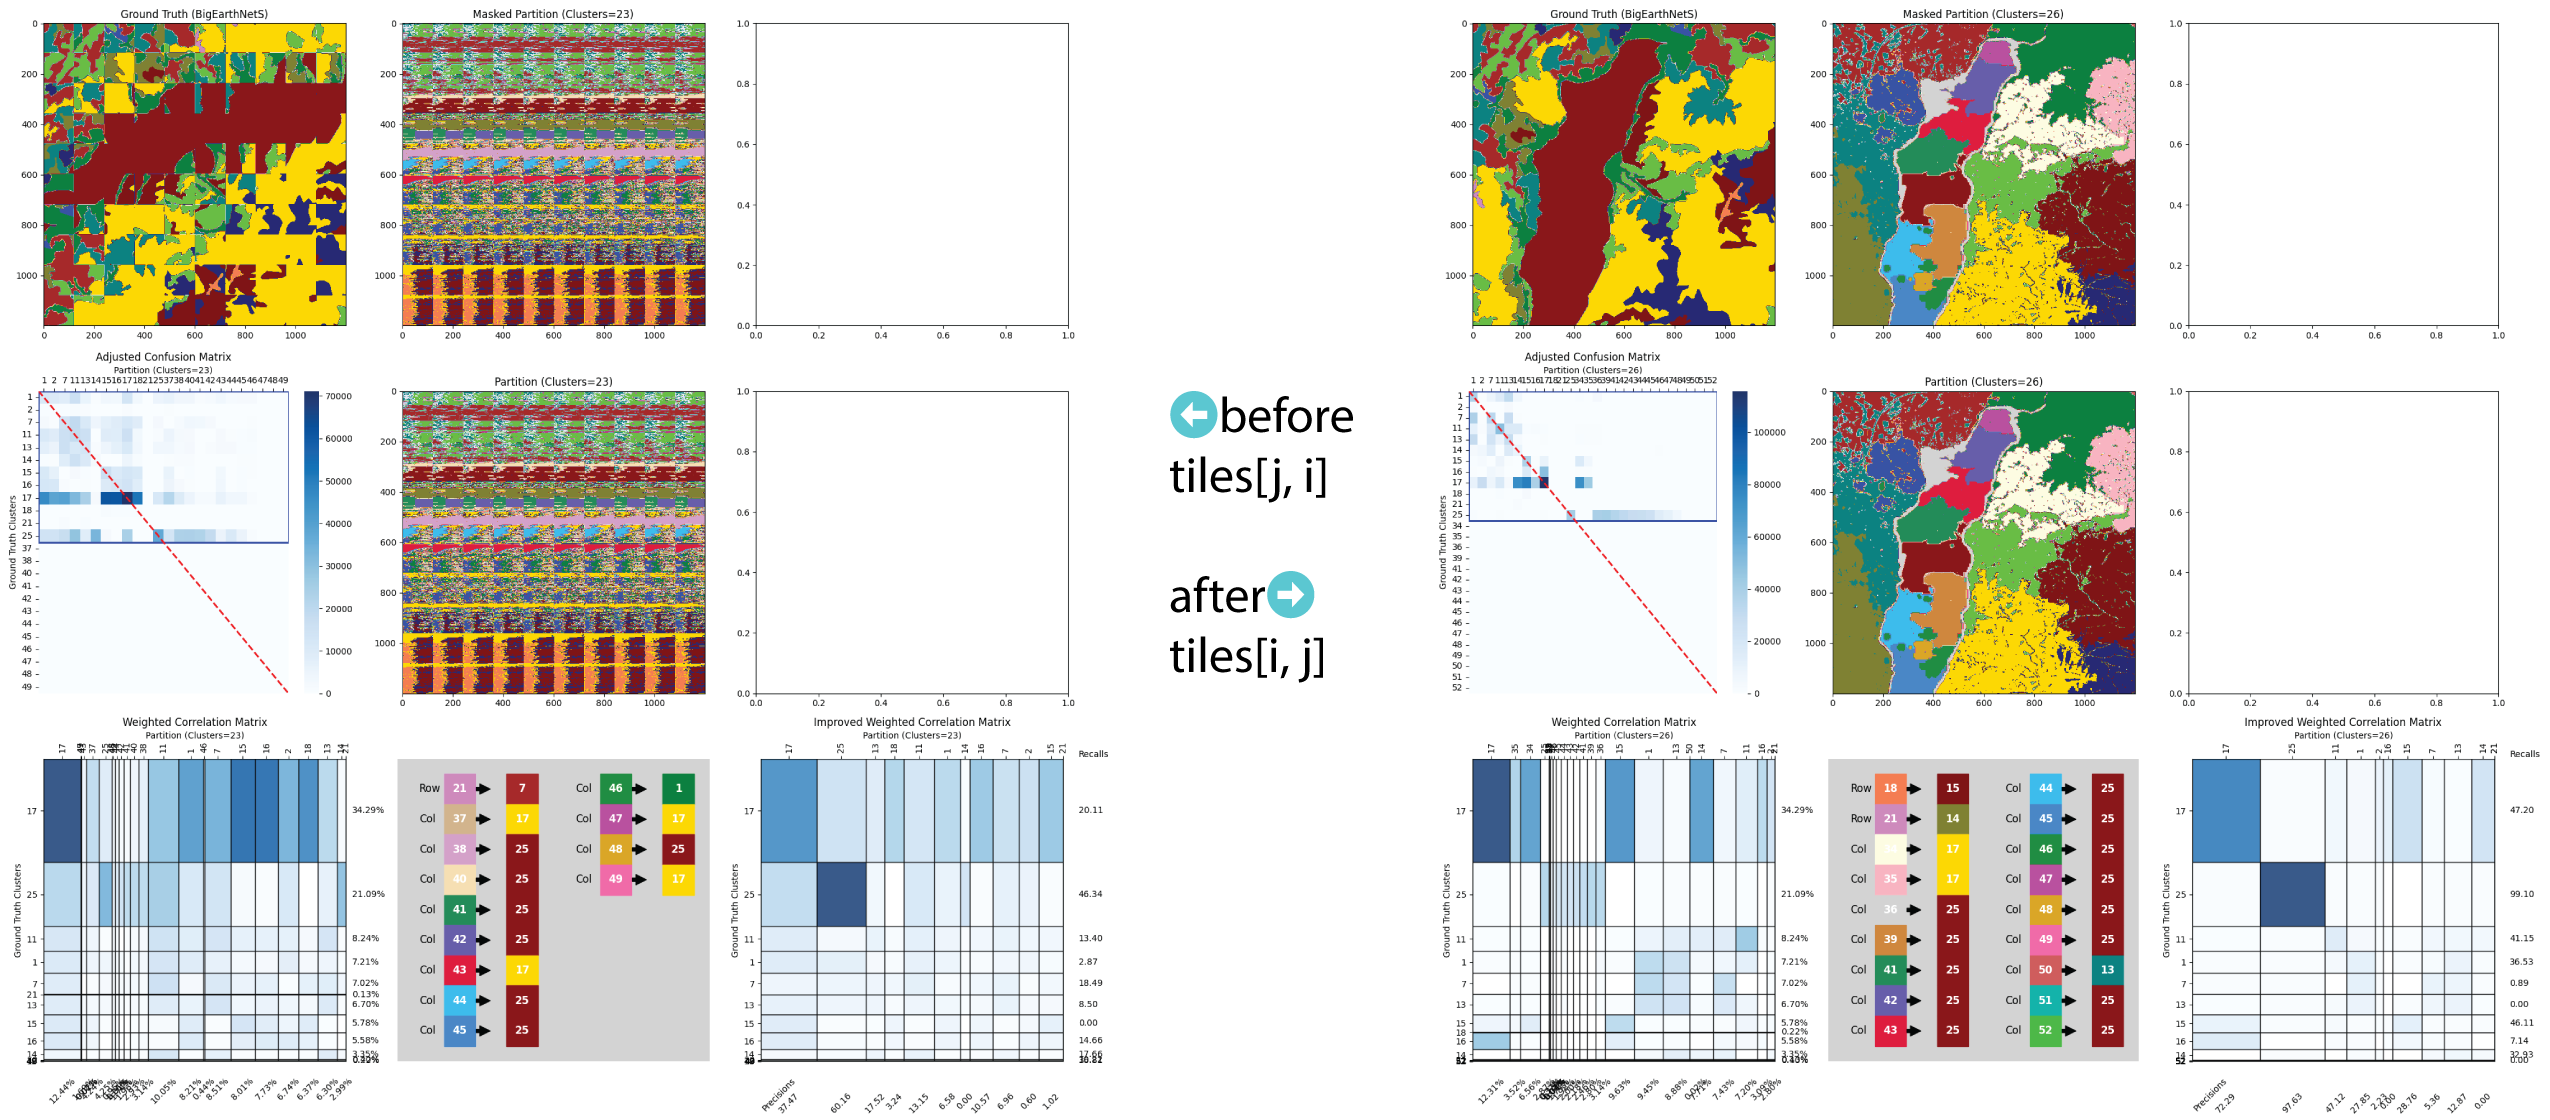
\includegraphics[width=\linewidth]{figures/24-10-07_BENimprove.png}
    \caption{(left) previous bad BEN example, using BlueRed, chose configuration with 23 clusters. (right) new BEN, using BlueRed, chosen configuration with 26 clusters. The improvement is made by "block transposing", i.e. define $tiles$ as a 10 by 10 array of tiles, swap $tiles[i,j]$ with $tiles[j,i]$ where $i,j \in [0,9]$ and $i,j \in Z$. Without, at least not identified, any changing any other implementation except the data loader, the periodic behavior was gone. \juntang[inline]{The reason for absence of periodic still not clear}} 
    \label{fig:24-10-07_BENimrove}
\end{figure}

\newpage

%%% =============================
%%% initial draft: Juntang Wang
%%% Oct. 07, 2024
%%% 